\section{Lagrange Mechanics}
\subsection{Euler-Lagrange equations}
The Lagrange function is defined as the difference between the kinetic energy $T$ and the potential energy $V$ of the system.
$$
\mathcal{L}=T(q,\dot{q})-V(q)=\frac{1}{2}{\dot{q}}^\top M\dot{q}-V(q)
$$
From the Lagrange function, we can derive the Euler-Lagrange equation by minimizing the "action integral" over the Lagrangian: (beyond the scope of this course)
$$
\frac{d}{dt}(\nabla_{\dot{q}}\mathcal{L})-\nabla_q\mathcal{L}=0 \qquad
\frac{d}{dt}(\nabla_{\dot{q}}T)-\nabla_q(T-V)=0
$$

\subsection{Generalized stuff}
\subsubsection{Generalized Coordinates}
\textbf{Definition:}

A set of time-dependent coordinates 
$$q(t)=\left[q_1,q_2,\cdots,q_n\right]^T$$
(that together with a set of fixed parameters) describes the configuration of the system at time $t$.
$q$ uniquely defines the position and orientation of the system.
\begin{itemize}
    \item A set q is generally not unique.
    \item The system’s degrees of freedom are the smallest number of generalized coordinates needed to represent the system.
\end{itemize}

\subsubsection{Generalized Kinetic Energy}
\begin{equation*}
    \begin{split}
        T(q,\dot{q})&=\frac{1}{2}mv^Tv+\frac{1}{2}\omega^TJ\omega\\
        T(q,\dot{q})&=\frac{1}{2}{\dot{q}}^\top M(q)\dot{q}
    \end{split}
\end{equation*}
Where $M$ is the mass inertia matrix, which can be calculated using logic or like this (where $p_i$ are point masses of mass $m_i$).

\begin{equation}
\begin{aligned}
% T = \sum\frac{1}{2}\dot{p_i}^Tm_i\dot{p_i} = \sum
%     \frac{1}{2}(\frac{\partial p}{\partial q}\frac{\partial q}{\partial t})^Tm_i(\frac{\partial p}{\partial q}\frac{\partial q}{\partial t}) \\ 
% T = \sum\frac{1}{2}\dot{q}^T(\frac{\partial p}{\partial q}^Tm_i\frac{\partial p}{\partial q})\dot{q}^T = \sum
%     \frac{1}{2}{\dot{q}}^\top M(q)\dot{q} \\
    M(q) = \sum\frac{\partial p_i}{\partial q}^Tm_i\frac{\partial p_i}{\partial q}
\end{aligned}
\end{equation}

\subsubsection{Generalized Potential Energy}
$$V(q)=mgh(q)+\frac{1}{2}k\Delta x^2(q)$$
\subsubsection{Generalized Forces}
% From $n$ masses/particles with displacement $r_i$ and a set of generalized coordinates $q=\left[q_1,q_2,\cdots,q_m\right]^\top$, the generalized force $Q$ is:
% $$
% Q=[Q_1,Q_2,\cdots,Q_m]^\top
% $$
% Where each element $Q_j$ is the force acting on the respective generalized coordinate $q_j$ and is given by:
% $$
% Q_j=\sum_{i=1}^{n}{F_i^\top\frac{\partial r_i}{\partial q_j}}
% $$
% The force $F_i$ acting on particle $r_i$ is written in terms of the displacement of particle $r_i$ in terms of the generalized coordinates. 
From $n$ masses/particles with displacement $r_i$ and a set of generalized coordinates $q=\left[q_1,q_2,\cdots,q_m\right]^\top$, the generalized force $Q$ is:
\begin{equation}\label{eq:generalized_force}
Q = \left(\frac{\partial \vec r}{\partial q}\right)^\top\vec F  
\end{equation}

where $F$ is a force or torque acting on the system, and $\vec r$ is the point of attack of the force.

The generalized forces $Q$ are then added to the r.h.s. of the Euler-Lagrange equations:
$$
\frac{d}{dt}\nabla_{\dot{q}}\mathcal{L}-\nabla_q\mathcal{L}=Q
$$

\textbf{Example:}\\
In \autoref{fig:generalized_force_ex} we see a force $F$ acting on a rod in 2D. Using \autoref{eq:generalized_force} we can find the generalized force $Q$ on the system. We see that the force acting in the $y$-direction results in a force on the $y$-part of $q$ and a torque equal $R\times F$. Just as we would expect from using other modeling techniques.
\begin{figure}[H]
    \centering
    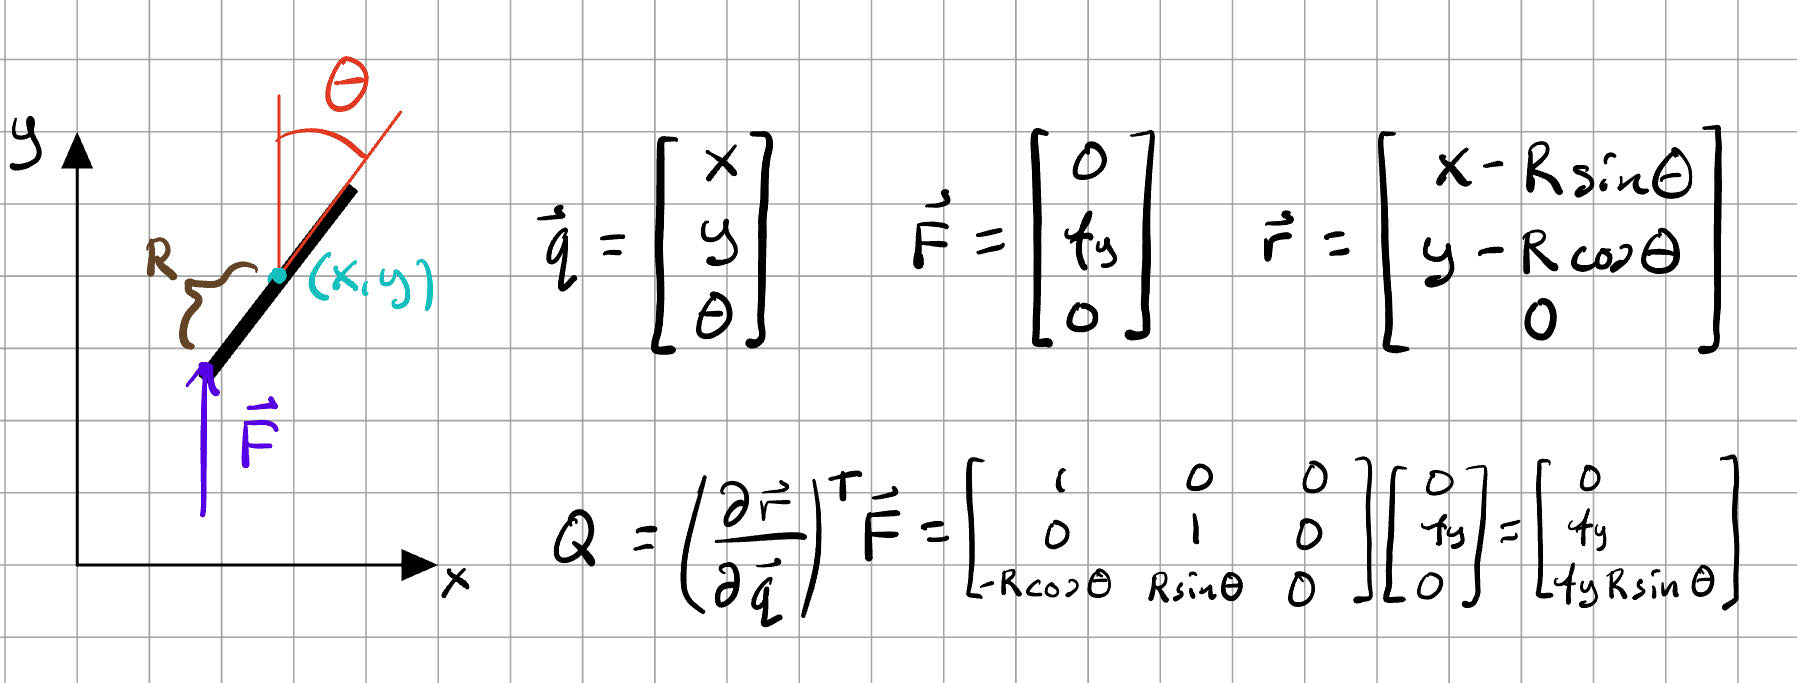
\includegraphics[scale=0.8]{figures/generalized forces example.png}
    \caption{Generalized force on a rotating rod in 2D-space}
    \label{fig:generalized_force_ex}
\end{figure}
\subsection{Mass Inertia Matrix}
The mass inertia matrix (or mass matrix) is a symmetric matrix $M$ that expresses the connection between the time derivative $\dot{q}$ of the generalized coordinate vector $q$ of a system and the kinetic energy $T$ of that system, by the equation:
$T=\frac{1}{2}\dot{q}M\dot{q}$
The mass matrix M can be found from the Lagrangian:
$$M=\nabla_{\dot{q}}^2\mathcal{L}$$
It is used in the Euler-Lagrange equations in place of the kinetic energy like this:
$$\nabla_{\dot{q}}\mathcal{L}=M\dot{q}$$
Sometimes $W$ is used instead of $M$. \\
\begin{tiny}
    All of the time in this course actually. It was stupid to use $M$ here.
\end{tiny}

\subsection{Lagrange Constraints}
If $\text{dim}(q)>\text{DOF}$ (Degrees of freedom) of the system, we need to add constraints to the Lagrangian. These constraints must be on the form $c(q)=0$.
With these constraints the Lagrangian now becomes
$\mathcal{L}=T-V-z^\top c$
Where $z$ is the Lagrangian multiplier (same as $\lambda$ in other classes).

Note: $z$ has as many elements as there are constraints.

The Lagrange and Euler-Lagrange equation now also takes the form,

\begin{equation}
    \mathcal{L}= T - V - z^\top c \qquad \frac{d}{dt}(\nabla_{\Dot{q}}T) - \nabla_{q}(T - V) + z\nabla_{q}c = Q 
\end{equation}

The sign of the last term on the left side of the equation can also be "$-$" but doesn't matter as $z$ changes to the "correct" sign based on choice.

\subsection{Lagrangian State-Space Formulation}

Using the Lagrange constraints, the system can be formulated as (lecture notes eq 2.168 pg. 50):

\begin{equation}
\label{eq:final_lagrange}
    \begin{bmatrix}
    M & \nabla_qc \\ \frac{\partial c}{\partial q} & 0
    \end{bmatrix}
    \begin{bmatrix}
    \ddot{q} \\ z
    \end{bmatrix}
    =
    \begin{bmatrix}
    Q-\dot{M}\dot{q}+\nabla_q (T-V) \\ 
    \frac{\partial }{\partial q}\left(\frac{\partial c}{\partial \dot{q}}\dot{q}\right)\dot{q}
    \end{bmatrix}
\end{equation}
where $\dot M(q) = \frac{\partial}{\partial q}(M(q)\dot q)$.

Here are some alternate ways to formulate as state space,

\begin{align*}
    \begin{split}
        x_1 &= q
        \\
        x_2 &= \Dot{q}
        \\
        \\
        \Dot{x}_1 &= x_2
        \\
        \Dot{x}_2 &= W^{-1}(x_1)\biggl[ Q + \underbrace{\nabla_{x_1} L}_\frac{\partial L}{\partial q} - \underbrace{\nabla_{x_1}(W(x_1)x_2)x_2}_{\frac{d}{dt}\cdot\frac{\partial T}{\partial \Dot{q}}} + z^\top \nabla c(x_1)\biggr]
    \end{split}
\end{align*}

The above equation can also be represented as semi-explicit DAE by using $\Dot{x}_2 = \Ddot{q}$ and constraint $c(x_1) = c(q)$ also known as equations of motion,

\begin{align*}
    \begin{split}
        W\Ddot{q} &= Q + \nabla_q L - \nabla_q \big[W(q)\Dot{q}\big]\Dot{q} + z^\top\nabla_q c(q)
        \\
        0 &= c(q)
    \end{split}
\end{align*}



\subsection{Index Reduction}

The following equation is a 3-index DAE. 
\begin{equation}
\label{eq:constrained_lagrange}
    \begin{aligned}
       \frac{d}{dt}\nabla_{\dot{q}}\mathcal{L}-\nabla_q\mathcal{L}&=Q \\
        c(q) &= 0 
    \end{aligned}
\end{equation}

in fact, all constrained Lagrange equations are of index 3, while unconstrained are of index 1.

% to equation \ref{eq:final_lagrange}, ie. 

% \begin{equation}
% \begin{aligned}
%    \frac{d}{dt}\nabla_{\dot{q}}\mathcal{L}-\nabla_q\mathcal{L}=Q \\
%     \ddot{c}(q) = 0 
% \end{aligned}
% \end{equation}

% you have taken a derivative twice, therefore equation \ref{eq:constrained_lagrange} is an index 3 DAE. 

\subsection{Baumgarte Stabilization}\label{section:Baumgarte}
Reducing the index of the Lagrangian gives the constraint $\ddot c(q) = 0$. This constraint is hard to enforce because numerical errors in the integration may generate noise and lead to low accuracy. This issue can be treated via Baumgarte stabilization, whereby the transformed model does not impose $\ddot c(q) = 0$, but rather dynamics on $c$ that stabilize them to zero. This can e.g. be done by imposing:
$$
\ddot c + 2\alpha \dot c + \alpha 2c = 0 
$$
where $\alpha>0$ is chosen such that the system is stable. The new model is:
\begin{equation*}
\begin{aligned}
\frac{d}{dt}\nabla_{\dot{q}}\mathcal{L}-\nabla_q\mathcal{L}&=Q \\
\ddot{c}+2 \alpha \dot{c}+\alpha^2 {c}&=0
\end{aligned}
\end{equation*}

\subsection{Important equations in lecture notes}

For the definition/alternative way to calculate W(q)=M(q) see eq. (2.6) pg. 18. 

For the non-constrained Lagrange, see eq. (2.109) pg. 37.

For the derivation and definition of generalized forces, see eq. (2.115) pg. 41. 

For the state-space version of constrained Lagrange, see eq. (2.168) pg. 50. 